\documentclass[11pt]{article}
\usepackage{algorithm2e}
\usepackage[italian]{babel}
\usepackage[document]{ragged2e}
\usepackage{amsfonts, amssymb, amsmath}
\usepackage{cancel}
\usepackage{float}
\usepackage{mathtools}
\usepackage[margin=3cm]{geometry}
\usepackage{subfig}
\usepackage{mwe}
\usepackage{hyperref}

\usepackage[
backend=biber,
sorting=none
]{biblatex}
\addbibresource{bibliografia.bib}

\tolerance=1
\emergencystretch=\maxdimen
\hyphenpenalty=10000
\hbadness=10000

\begin{document}
\graphicspath{ {./img/} }
\begin{titlepage}
    \begin{center}
        \vspace*{1.5cm}
            
        \Huge
        \textbf{IMAGING} \\
        \LARGE
        Deblur
                        
        \vspace{2.0cm}
          
        \begin{minipage}[t]{0.47\textwidth}
        \begin{center}
        	{\large{\bf Cheikh Ibrahim $\cdot$ Zaid}}\\
			{\large Matricola: \texttt{0000974909}}
        \end{center}

		\end{minipage}
		\hfill
		\begin{minipage}[t]{0.47\textwidth}\raggedleft
		\begin{center}
        	{\large{\bf Xia $\cdot$ Tian Cheng}}\\
			{\large Matricola: \texttt{0000975129}}
        \end{center}
		\end{minipage}  
            
        \vspace{6cm}
            
        Anno accademico\\
        $2021 - 2022$
            
        \vspace{0.8cm}
            
            
        \Large
        Corso di Calcolo Numerico\\
        Alma Mater Studiorum $\cdot$ Università di Bologna\\
            
    \end{center}
\end{titlepage}
\pagebreak

\tableofcontents
\newpage

\section{Introduzione}
Il progetto consiste nel ricostruire un'immagine a partire da una sua istanza alterata da uno sfocamento noto e un rumore casuale.\\
Si tratta di un problema solitamente affrontato elaborando immagini provenienti da un dispositivo di acquisizione che, nel suo processo di formazione, altera la figura originale producendo un risultato diverso dalla realtà.\\ 
La soluzione di tale problema viene formulata come problema ai minimi quadrati:
\begin{align*}
    \min\limits_{x} \frac{1}{2} \Vert Ax-b \|_{2}^{2}
\end{align*}
dove $A$ è l'operatore di blur, $x$ l'immagine ricostruita e $b$ l'immagine acquisita.\\

Per la risoluzione sono note diverse formulazioni. Quelle impiegate sono:
\begin{itemize}
    \setlength\itemsep{0.05cm}
    \item Metodo naive, risolvendo il problema in modo diretto. Questo approccio è noto essere mal condizionato.
    \item Regolarizzazione di Tikhonov:
    \begin{align*}
    	\min\limits_{x} \frac{1}{2} \Vert Ax-b \|_{2}^{2} + \lambda \Vert x \|_{2}^{2}
    \end{align*}
    \item Regolarizzazione tramite variazione totale:
    \begin{align*}
    	\min\limits_{x} \frac{1}{2} \Vert Ax-b \|_{2}^{2} + \lambda \phi_{\text{TV}}(x)
    \end{align*}

\end{itemize}
Per misurare la qualità dei risultati verranno impiegate due metriche:
\begin{itemize}
    \setlength\itemsep{0.05cm}
    \item Mean Squared Error (MSE): un valore sempre positivo usato per stimare l'errore tra due oggetti. \\
    L'impiego del quadrato permette di "esagerare" il risultato ottenuto in presenza di errori elevati e di minimizzarlo in presenza di errori piccoli.
    \item Peak Signal-to-Noise Ratio (PSNR): una metrica usata per valutare la qualità di ricostruzione di un'immagine o un video. Per due immagini identiche, il $\text{PSNR}=\infty$, quindi maggiore è il PSNR, maggiore è la vicinanza tra le immagini confrontate.\\
	Ci si aspetta, inoltre, che il valore del MSE e PSNR siano correlati, dal momento che la formula per calcolare il PSNR si basa sul valore del MSE.
\end{itemize}




\newpage
\section{Esecuzione preliminare}
\label{chap:lambda}
Per avere una visione sul comportamento delle varie formulazioni, sono state eseguite delle prime sperimentazioni sull'immagine in \autoref{fig:originale1}.
\begin{figure}[H]
    \centering
    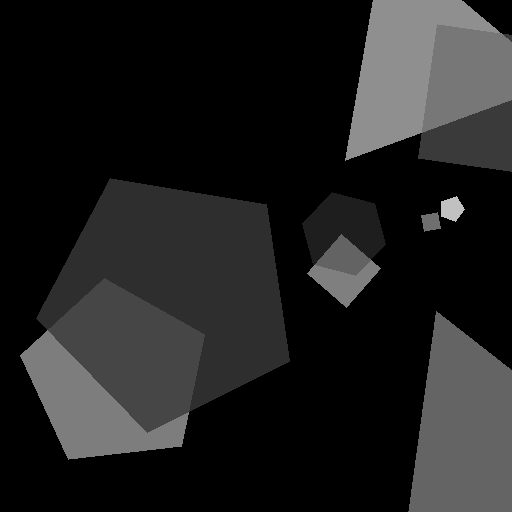
\includegraphics[width=4cm]{esecuzione/originale.png}
    \caption{Immagine di test}
    \label{fig:originale1}
\end{figure}

\subsection{Determinare il valore di lambda}
Prima di eseguire i metodi, è necessario determinare il valore $\lambda$ del parametro di regolarizzazione dei metodi che lo prevedono.\\
Esistono condizioni che permettono di determinare un valore di $\lambda$ accettabile (\textit{es. principio della discrepanza di Morozov}). In questo progetto verrà stimato utilizzando una ricerca iterativa del punto migliore basato sul PSNR (funzione \texttt{search\_best\_lambda} nel sorgente).

\subsection{Prima esecuzione}
La prima esecuzione è stata effettuata con un blur generato da un kernel $5 \times 5$ con $\sigma=0.5$ e rumore gaussiano con deviazione standard $0.05$.

\subsubsection{Stima di lambda}
Il seguente grafico mostra il valore del PSNR al variare di $\lambda \in [0.01, 1[$ con passo $0.01$ per la regolarizzazione di Tikhonov:
\begin{figure}[H]
    \centering
    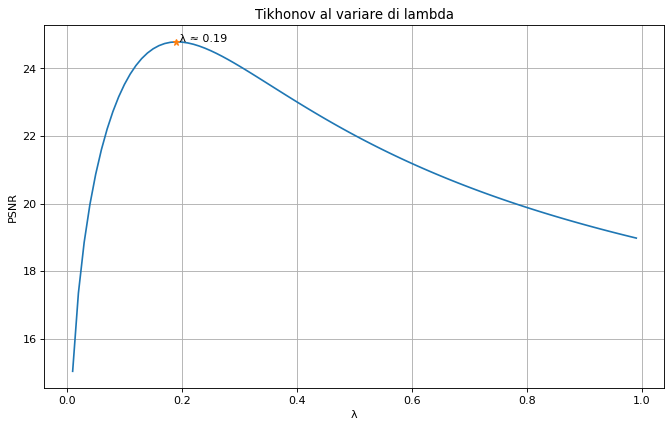
\includegraphics[width=8.5cm]{esecuzione/1/tikhonov_lambda.png}
    \caption{$\lambda=0.19$ e $\texttt{PSNR} \simeq 24.79$}
    \label{fig:tikhonov_lambda1}
\end{figure}
Analogamente, il seguente grafico mostra la variazione del PSNR per $\lambda \in [0.01, 1[$ con passo $0.01$ per la regolarizzazione tramite variazione totale:
\begin{figure}[H]
    \centering
    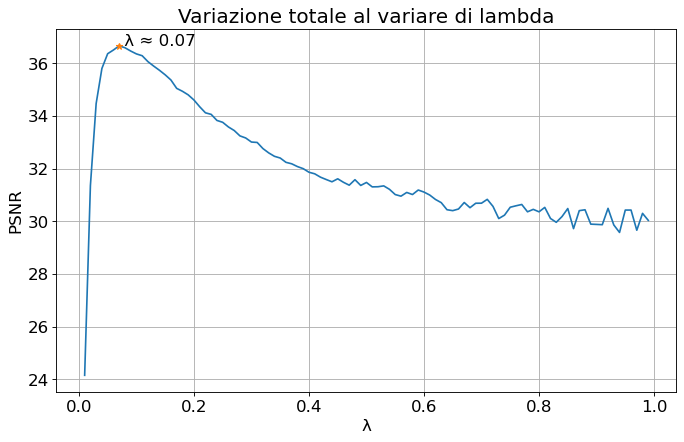
\includegraphics[width=8.5cm]{esecuzione/1/tv_lambda.png}
    \caption{$\lambda=0.07$ e $\texttt{PSNR} \simeq 36.74$}
    \label{fig:tv_lambda1}
\end{figure}	

\subsubsection{Risultato}
Fissati i valori di $\lambda$, il risultato ottenuto è il seguente:\\
\begin{figure}[H]
    \centering
    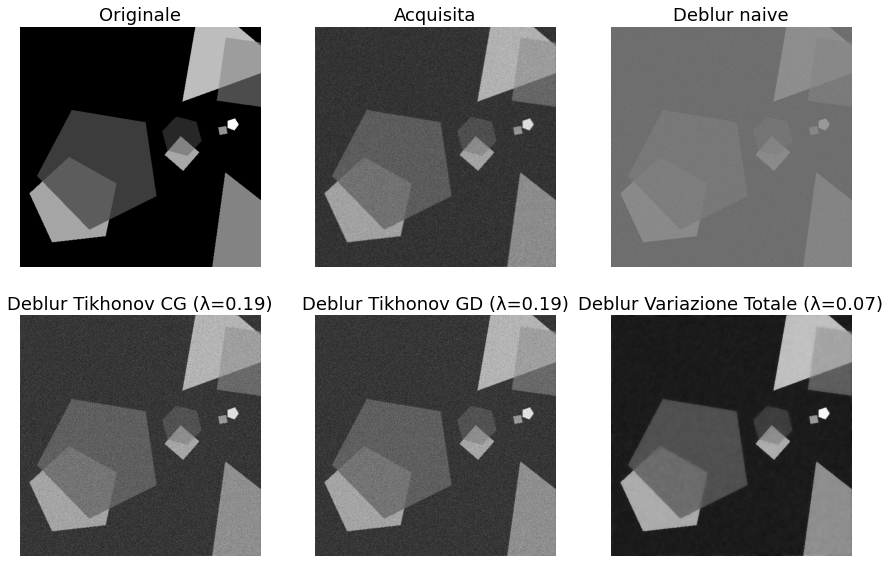
\includegraphics[width=15cm]{esecuzione/1/deblur.png}
    \caption{Risultato del processo di deblur}
    \label{fig:deblur1}
\end{figure}

\begin{center}
    \begin{tabular}{ |c|c|c|c|c|c| }
    \hline
    & Acquisita & Naive & Tikhonov CG & Tikhonov GD & Variazione totale \\ 
    \hline
    MSE & $0.2699 \cdot 10^{-2}$ & $0.2047 \cdot 10^{0}$ & $0.3320 \cdot 10^{-2}$ & $0.3320 \cdot 10^{-2}$ & $0.2119 \cdot 10^{-3}$ \\ 
    PSNR & $25.6878$ & $6.8874$ & $24.7890$ & $24.7890$ & $36.7382$ \\ 
    Iter. & & 140 & 14 & 48 & 14 \\ 
    \hline
    \end{tabular}
\end{center}

Come atteso, la ricostruzione ottenuta con la formulazione come problema ai minimi quadrati senza regolarizzazione ha prodotto un'immagine molto distante dall'originale.\\
Utilizzando la regolarizzazione di Tikhonov, si è ottenuto un risultato quasi invariato rispetto all'immagine acquisita, se non addirittura peggiore.\\
Invece, con la regolarizzazione tramite variazione totale, il risultato ottenuto è migliore rispetto agli altri metodi e visivamente molto vicina all'immagine originale.\\~\\
A livello di velocità, minimizzare con il metodo del gradiente ha richiesto più iterazioni rispetto al metodo del gradiente coniugato. \\
Invece, a parità di numero di iterazioni, il metodo regolarizzato con Tikhonov ha richiesto meno tempo rispetto al metodo che utilizza variazione totale. Si tratta di un risultato atteso considerando che il termine di regolarizzazione $\phi_{\text{TV}}$ è molto più articolato rispetto a quello di Tikhonov.


\subsection{Seconda esecuzione}
Per vedere le prestazioni in uno scenario differente, è stata effettuata una seconda esecuzione sulla stessa immagine di partenza con blur ottenuto da un kernel $25 \times 25$ con $\sigma=3$ e rumore con deviazione standard $0.05$.

\subsubsection{Stima di lambda}
\begin{figure}[H]
    \centering
    \begin{minipage}{0.45\textwidth}
        \centering
        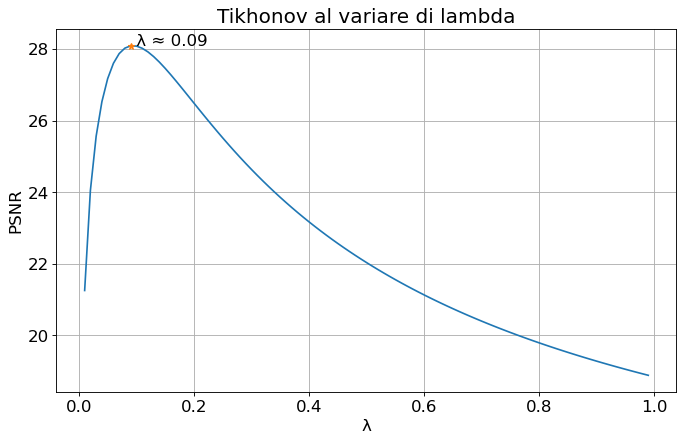
\includegraphics[width=7.5cm]{esecuzione/2/tikhonov_lambda.png}
        \caption{$\lambda=0.09$ e $\texttt{PSNR} \simeq 28.09$}
        \label{fig:tikhonov_lambda2}
    \end{minipage}\hfill
    \begin{minipage}{0.45\textwidth}
        \centering
        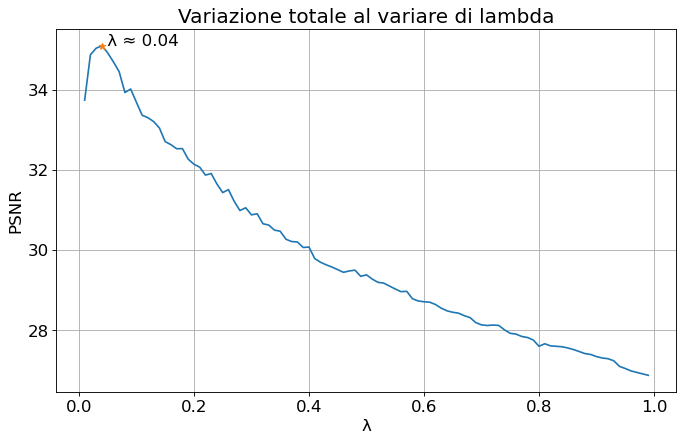
\includegraphics[width=7.5cm]{esecuzione/2/tv_lambda.png}
        \caption{$\lambda=0.04$ e $\texttt{PSNR} \simeq 35.09$}
        \label{fig:tv_lambda2}
    \end{minipage}
\end{figure}

\subsubsection{Risultato}
\begin{figure}[H]
    \centering
    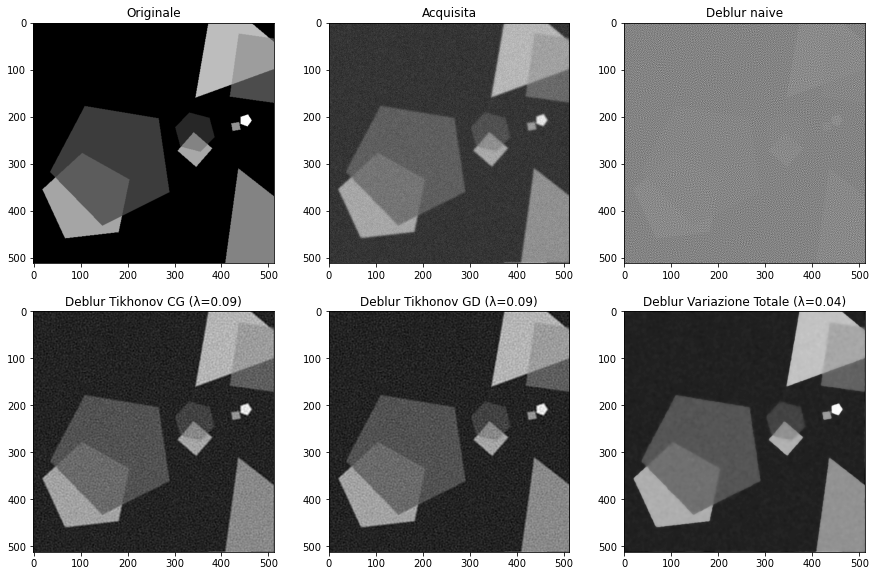
\includegraphics[width=15cm]{esecuzione/2/deblur.png}
    \caption{Risultato del processo di deblur}
    \label{fig:deblur2}
\end{figure}

\begin{center}
    \begin{tabular}{ |c|c|c|c|c|c| }
    \hline
    & Acquisita & Naive & Tikhonov CG & Tikhonov GD & Variazione totale \\ 
    \hline
    MSE & $0.3204 \cdot 10^{-2}$ & $0.5719 \cdot 10^{-1}$ & $0.1553 \cdot 10^{-2}$ & $0.1553 \cdot 10^{-2}$ & $0.3094 \cdot 10^{-3}$ \\ 
    PSNR & $24.9437$ & $-7.5735$ & $28.0889$ & $28.0890$ & $35.0944$ \\ 
    Iter. & & 200 (max) & 18 & 99 & 29 \\ 
    \hline
    \end{tabular}
\end{center}

Anche in questo caso, il metodo naive non ha prodotto soluzioni accettabili, mentre la regolarizzazione tramite variazione totale ha prodotto il risultato migliore.\\
Il metodo regolarizzato con Tikhonov, a differenza dell'esecuzione precedente, ha prodotto un risultato migliore dell'immagine acquisita mentre a livello di velocità, analogamente al caso precedente, minimizzare con il gradiente coniugato ha richiesto meno iterazioni rispetto al metodo del gradiente.




\newpage
\section{Confronto tra gradiente coniugato e metodo del gradiente}
\label{chap:confronto}
Si analizzano ora, in modo più approfondito, le prestazioni di Tikhonov utilizzando i due metodi di discesa implementati, focalizzando l'attenzione sulla velocità e precisione. \\

\subsection{Prima esecuzione}
Per una prima sperimentazione si è usata la \autoref{fig:originale1} con kernel $5 \times 5$ con $\sigma=0.5$ e rumore gaussiano con deviazione standard $0.05$.\\
I risultati ottenuti sono i seguenti:
\begin{figure}[H]
    \centering
    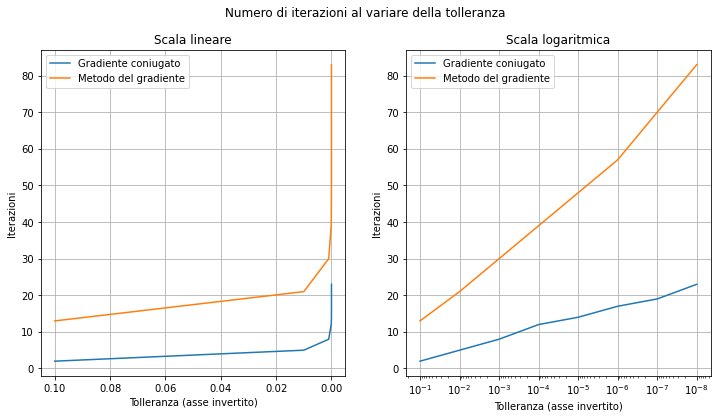
\includegraphics[width=11cm]{iterazioni_cg_gd/1/tol_iter.png}
    \caption{Numero di iterazioni al variare della tolleranza}
    \label{fig:tol_iter1}
\end{figure}
È immediato notare, in linea con le osservazioni precedenti, che il metodo del gradiente coniugato necessita di meno iterazioni rispetto al metodo del gradiente prima di raggiungere le condizioni di convergenza.\\

\begin{figure}[H]
    \centering
    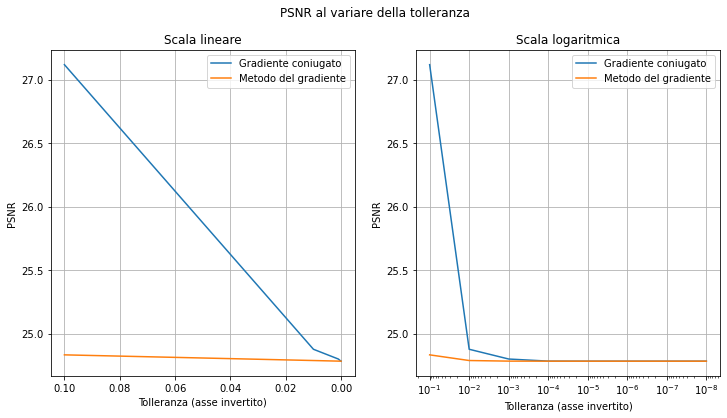
\includegraphics[width=11cm]{iterazioni_cg_gd/1/tol_psnr.png}
    \caption{PSNR al variare della tolleranza}
    \label{fig:tol_psnr1}
\end{figure}
A livello di precisione, invece, il risultato ottenuto mostra che i due metodi, al variare della tolleranza, convergono intorno allo stesso risultato.\\
È però presente un comportamento controintuitivo in vicinanza di valori di tolleranza elevati dove si ottiene un PSNR maggiore.
In altri termini, si ottiene un'immagine più fedele all'originale con meno iterazioni, mentre il risultato peggiora nella continuazione dell'esecuzione (tale problematica verrà approfondita nella \autoref{chap:semiconv}).

\begin{figure}[H]
    \centering
    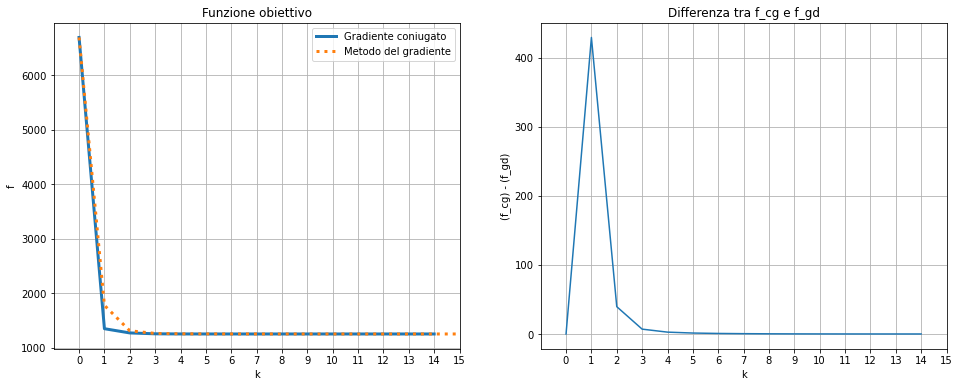
\includegraphics[width=14cm]{iterazioni_cg_gd/1/funzione_obiettivo.png}
    \caption{Andamento della funzione obiettivo}
    \label{fig:obiettivo1}
\end{figure}
\begin{figure}[H]
    \centering
    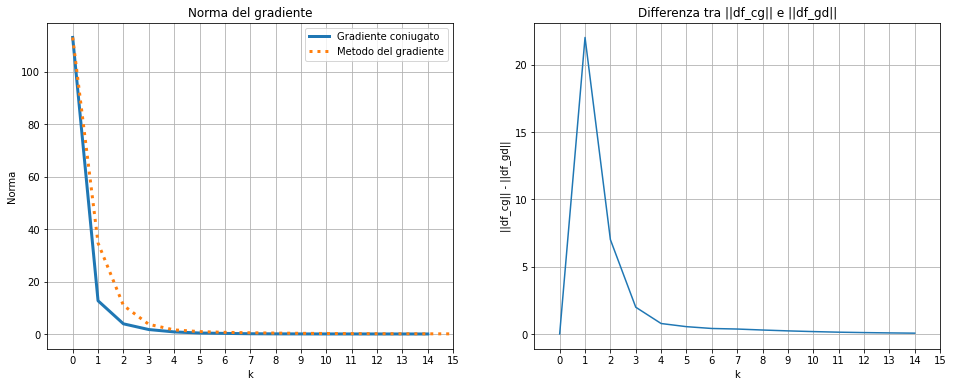
\includegraphics[width=14cm]{iterazioni_cg_gd/1/norma_gradiente.png}
    \caption{Andamento della norma del gradiente}
    \label{fig:gradiente1}
\end{figure}
Infine, come atteso dai risultati precedenti, per il metodo del gradiente coniugato la decrescita della funzione obiettivo è maggiore rispetto al metodo del gradiente. 
Lo stesso risultato è osservabile con la norma del gradente che nel caso del gradiente coniugato esegue passi di dimensione maggiore.

\subsection{Seconda esecuzione}
Per una seconda valutazione si è usato un kernel $25 \times 25$ con $\sigma=3$ e rumore gaussiano con deviazione standard $0.05$.\\

\begin{figure}[H]
    \centering
    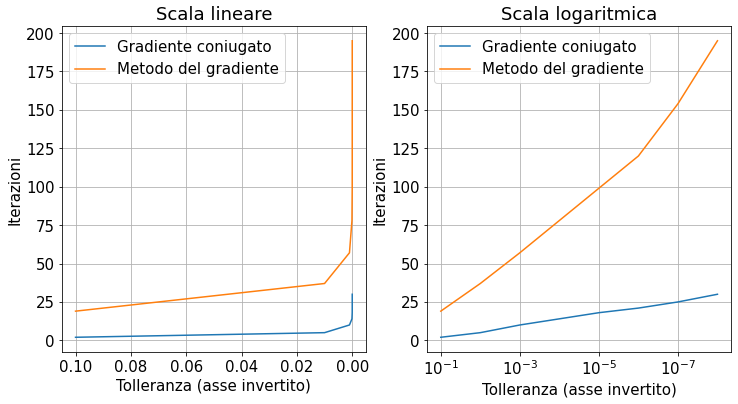
\includegraphics[width=11cm]{iterazioni_cg_gd/2/tol_iter.png}
    \caption{Numero di iterazioni al variare della tolleranza}
    \label{fig:tol_iter2}
\end{figure}
\begin{figure}[H]
    \centering
    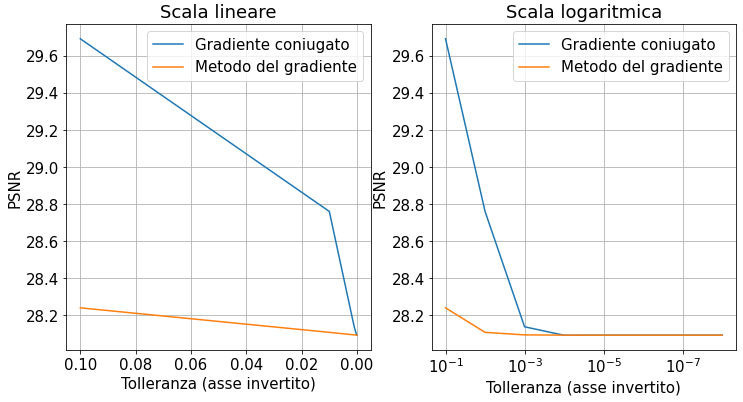
\includegraphics[width=11cm]{iterazioni_cg_gd/2/tol_psnr.png}
    \caption{PSNR al variare della tolleranza}
    \label{fig:tol_psnr2}
\end{figure}
\begin{figure}[H]
    \centering
    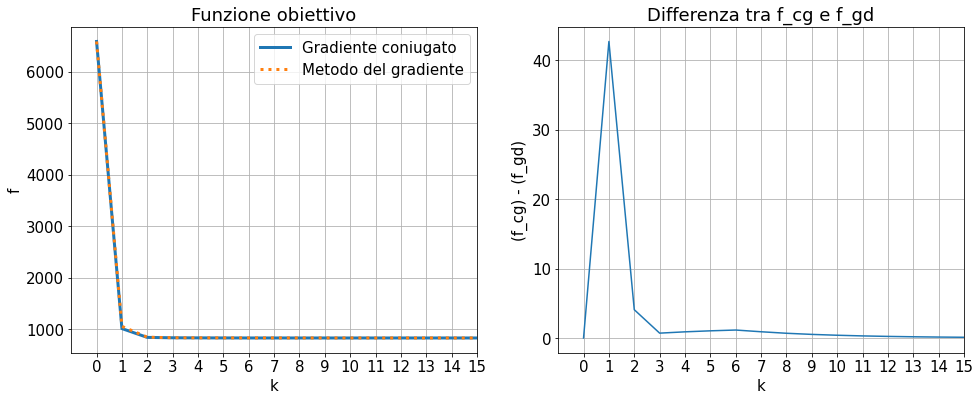
\includegraphics[width=14cm]{iterazioni_cg_gd/2/funzione_obiettivo.png}
    \caption{Andamento della funzione obiettivo}
    \label{fig:obiettivo2}
\end{figure}
\begin{figure}[H]
    \centering
    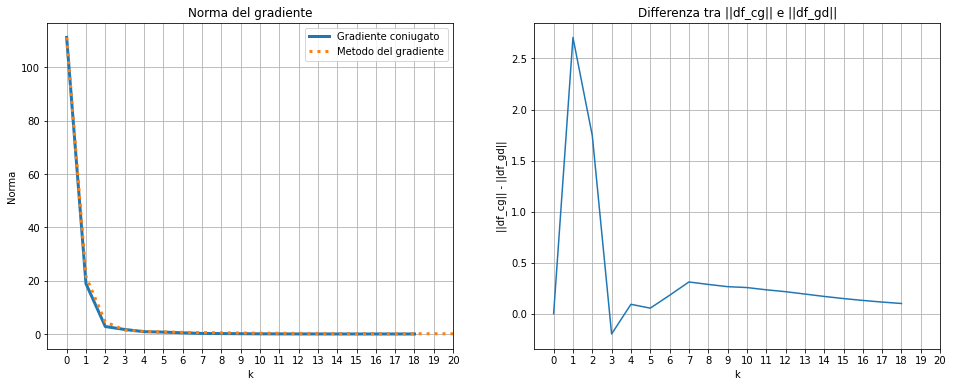
\includegraphics[width=14cm]{iterazioni_cg_gd/2/norma_gradiente.png}
    \caption{Andamento della norma del gradiente}
    \label{fig:gradiente2}
\end{figure}

I risultati ottenuti sono in linea con quelli precedenti ed evidenziano che le prestazioni del gradiente coniugato sono maggiori rispetto a quelle del metodo del gradiente, 
come atteso dalle analisi teoriche. Infatti, le immagini utilizzate sono a sfondo omogeneo e tendono ad essere molto vicine alla forma di una matrice sparsa per la quale il metodo del gradiente coniugato ha buone prestazioni.\\
La soluzione calcolata invece, escludendo valori di tolleranza elevati, converge intorno allo stesso valore e per questo motivo è, in generale, indifferente utilizzare l'implementazione del deblur con i due metodi di discesa. Ovviamente per questioni di velocità, si preferisce utilizzare il metodo implementato con il gradiente coniugato.




\newpage
\section{Semi-convergenza}
\label{chap:semiconv}
Nella \autoref{chap:confronto} è emerso il problema per cui l'immagine ottenuta con meno iterazioni è qualitativamente migliore rispetto a quella ottenuta quando il metodo raggiunge convergenza. 
Tale problema è noto come semi-convergenza \cite{1}\cite{2}\cite{3}, ovvero quando il raggiungimento dell'ottimo non corrisponde al soddisfacimento delle condizioni di convergenza e per questo le iterazioni successive peggiorano il risultato.\\
Nel contesto del deblur, il problema di semi-convergenza è causato dal rumore aggiunto all'immagine. È noto che il metodo naive è quello che più viene condizionato dal rumore e per questa ragione vengono introdotti i metodi di regolarizzazione.\\
Si analizzano quindi i risultati dei vari metodi valutando l'andamento del PSNR rispetto all'iterato $x_{k}$:

\subsection{Analisi con rumore}
\subsubsection{Metodo naive}
\begin{figure}[H]
    \centering
    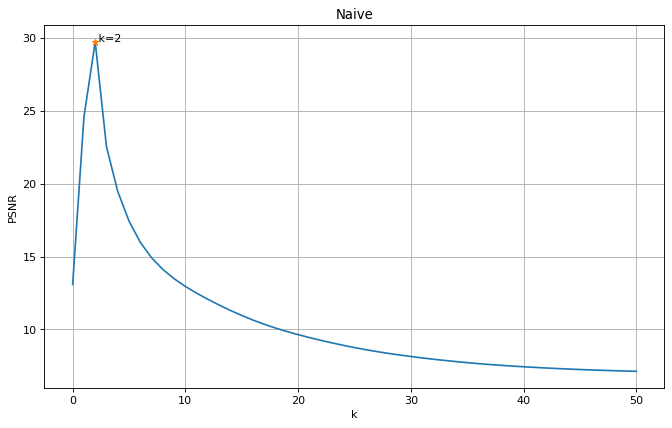
\includegraphics[width=8cm]{semiconvergenza/1/psnr_naive.png}
    \caption{PSNR al variare dell'iterato $x_k$}
    \label{fig:semiconv_psnr_naive1}
\end{figure}
\begin{figure}[H]
    \centering
    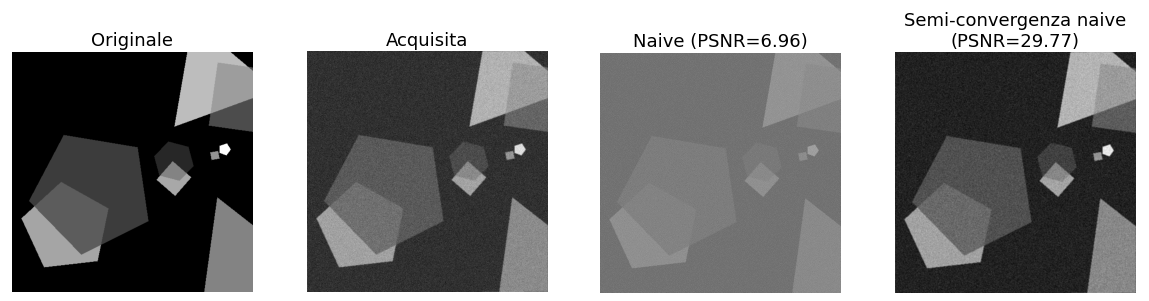
\includegraphics[width=15cm]{semiconvergenza/1/deblur_naive.png}
    \caption{Risultato ottenuto}
    \label{fig:semiconv_deblur_naive1}
\end{figure}
Come atteso, il risultato viene distorto molto rapidamente e in maniera molto drastica. Quindi, al raggiungimento delle condizioni di convergenza, il risultato ottenuto è inevitabilmente molto distante dall'immagine reale.\\
Terminando l'esecuzione al punto di massimo invece, il risultato è una buona ricostruzione dell'immagine reale e, in questo caso, anche migliore rispetto alla soluzione del metodo regolarizzato con Tikhonov in \autoref{chap:lambda}.

\subsubsection{Regolarizzazione di Tikhonov}
\begin{figure}[H]
    \centering
    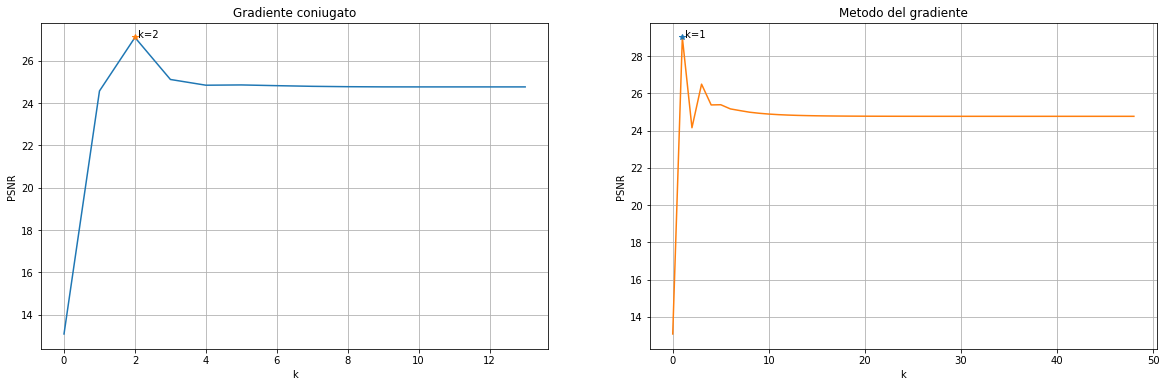
\includegraphics[width=15cm]{semiconvergenza/1/psnr_tikhonov.png}
    \caption{PSNR al variare dell'iterato $x_k$}
    \label{fig:semiconv_psnr_tikhonov1}
\end{figure}
\begin{figure}[H]
    \centering
    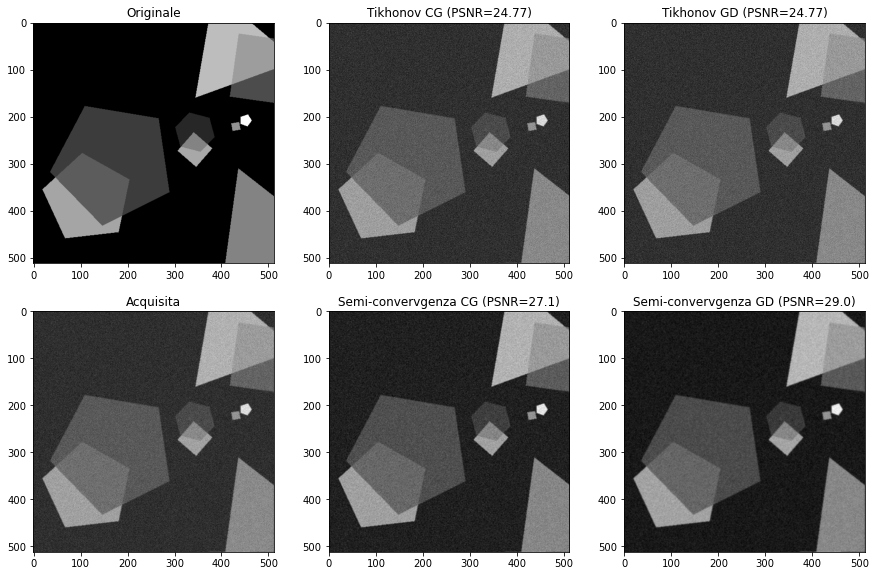
\includegraphics[width=10cm]{semiconvergenza/1/deblur_tikhonov.png}
    \caption{Risultato ottenuto}
    \label{fig:semiconv_deblur_tikhonov1}
\end{figure}
Con la regolarizzazione di Tikhonov si nota che, nonostante sia ancora presente il problema di semi-convergenza, dopo il punto di ottimo l'errore decresce di una quantità più contenuta rispetto al metodo naive fino ad assumere un comportamento asintotico.\\
Anche in questo caso però, confrontando il risultato al punto di semi-convergenza e convergenza si nota, in una forma meno grave rispetto al metodo naive, una differenza significativa.

\subsubsection{Regolarizzazione tramite variazione totale}
\begin{figure}[H]
    \centering
    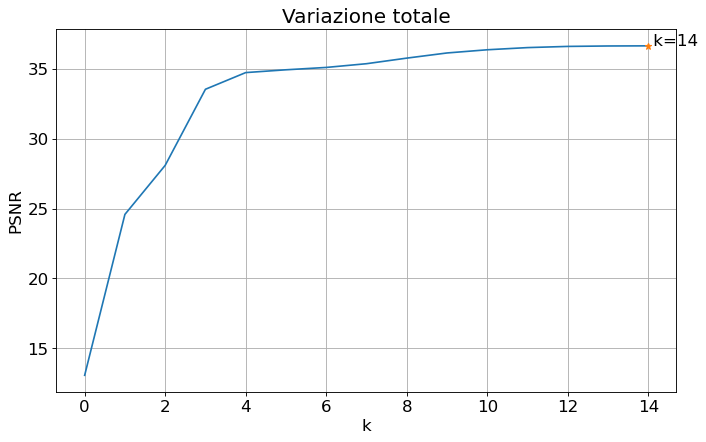
\includegraphics[width=9cm]{semiconvergenza/1/psnr_tv.png}
    \caption{PSNR al variare dell'iterato $x_k$}
    \label{fig:semiconv_psnr_tv1}
\end{figure}
\begin{figure}[H]
    \centering
    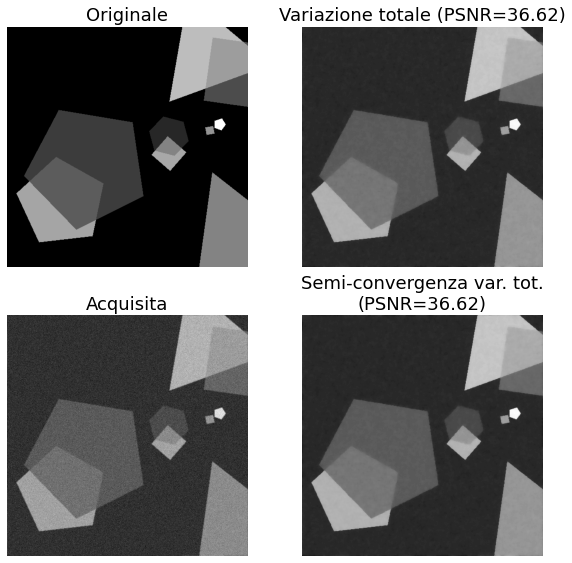
\includegraphics[width=15cm]{semiconvergenza/1/deblur_tv.png}
    \caption{Risultato ottenuto}
    \label{fig:semiconv_deblur_tv1}
\end{figure}
Regolarizzando tramite variazione totale, invece, il problema di semi-convergenza è assente nel caso dell'immagine analizzata e il raggiungimento dell'ottimo avviene contemporaneamente al soddisfacimento delle condizioni di convergenza.

\subsubsection{Risultato}
Le prove precedenti sono state eseguite con kernel $5 \times 5$ con $\sigma=0.5$ e kernel $25 \times 25$ con $\sigma=3$, entrambi i casi applicando un rumore con deviazione standard $0.05$.\\
La regolarizzazione tramite variazione totale si è rivelata la soluzione meno soggetta alla semi-convergenza, mentre Tikhonov, nonostante non restituisca la soluzione del punto ottimo, è in grado di ridurre significativamente il deterioramento della soluzione.\\~\\
Nel caso generale, non è però possibile risolvere il problema di semi-convergenza interrompendo l'esecuzione quando si rileva un punto di massimo. 
Un controesempio è il caso del metodo del gradiente in \autoref{fig:semiconv_psnr_tikhonov1}, infatti, l'andamento del PSNR può assume più punti di massimo locale e quindi esisteranno casi in cui il primo massimo raggiunto non sarà necessariamente la soluzione ottima.

\subsection{Analisi senza rumore}
Si eseguono ora gli stessi esperimenti su un'immagine a cui è stato applicato un blur senza aggiungere rumore.\\
Un aspetto da tenere in considerazione è che la ricerca del parametro di regolarizzazione $\lambda$ ha prodotto risultati tendenti a 0. Per evitare di annullare il termine di regolarizzazione, riconducendosi al metodo naive, è stato scelto un valore di $\lambda$ molto piccolo.

\begin{figure}[H]
    \centering
    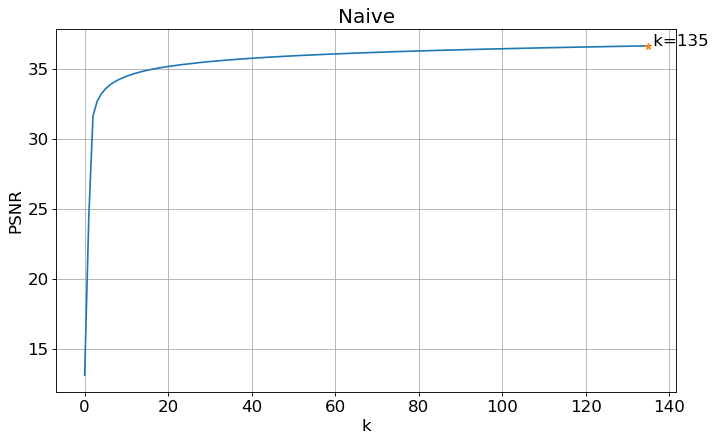
\includegraphics[width=8cm]{semiconvergenza/3/psnr_naive.png}
    \caption{PSNR al variare dell'iterato $x_k$ con il metodo naive}
    \label{fig:semiconv_psnr_naive3}
\end{figure}
\begin{figure}[H]
    \centering
    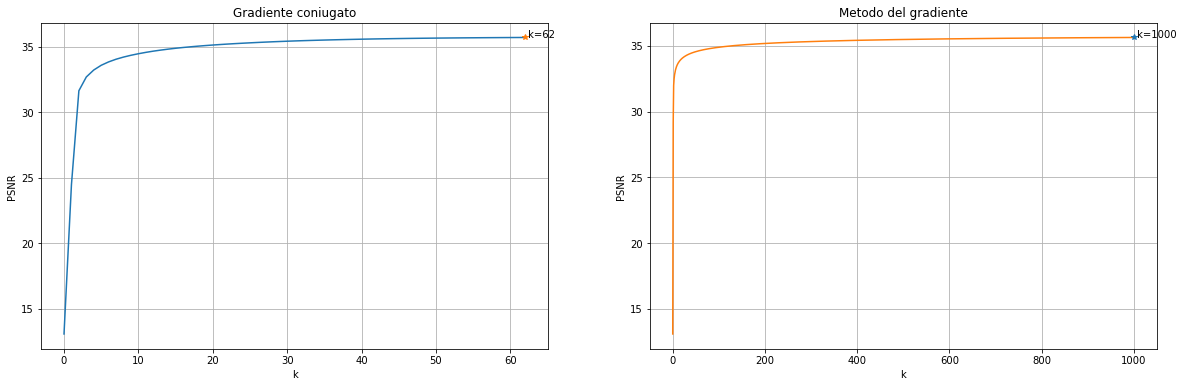
\includegraphics[width=13cm]{semiconvergenza/3/psnr_tikhonov.png}
    \caption{PSNR al variare dell'iterato $x_k$ con regolarizzazione di Tikhonov}
    \label{fig:semiconv_deblur_tikhonov3}
\end{figure}
\begin{figure}[H]
    \centering
    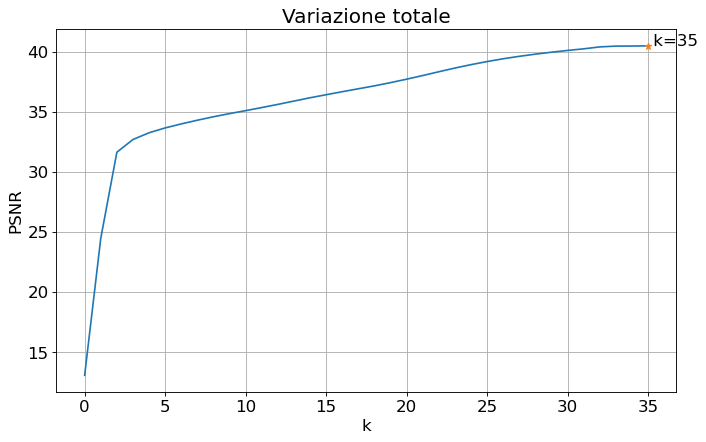
\includegraphics[width=8cm]{semiconvergenza/3/psnr_tv.png}
    \caption{PSNR al variare dell'iterato $x_k$ con regolarizzazione tramite variazione totale}
    \label{fig:semiconv_deblur_tv3}
\end{figure}
\begin{figure}[H]
    \centering
    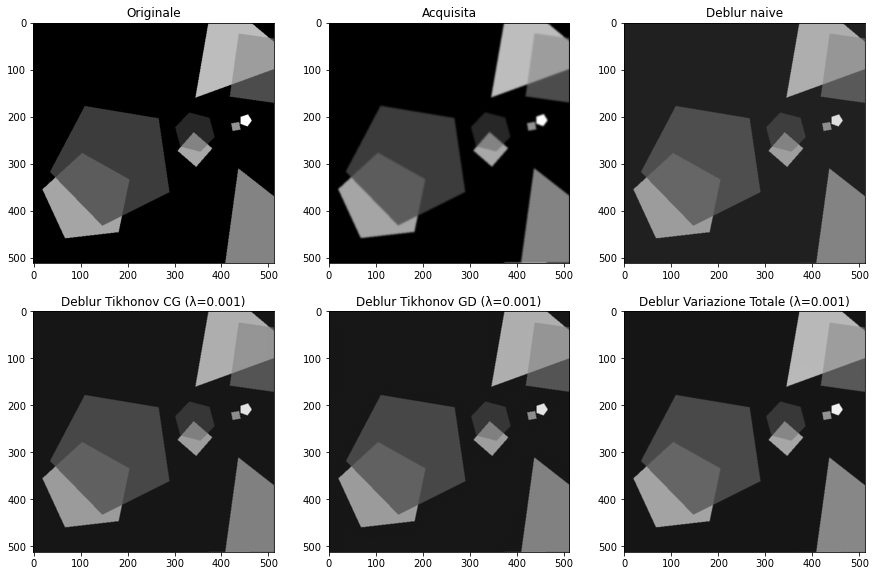
\includegraphics[width=12cm]{semiconvergenza/3/deblur_all.png}
    \caption{Risultato ottenuto}
    \label{fig:semiconv_deblur3}
\end{figure}
In questo caso, tutti i metodi hanno raggiunto convergenza e ottimo contemporaneamente e il risultato, in assenza di rumore, si presenta visivamente molto simile indipendentemente dalla formulazione.



\newpage
\section{Risultati su esecuzioni multiple}
\subsection{Esecuzioni su immagini generate casualmente}
Per una valutazione più generalizzata dei metodi, sono stati eseguiti dei test su un dataset di immagini contenenti poligoni regolari generati casualmente (funzione \texttt{generate\_image} del sorgente)
a cui è stato applicato un blur con kernel $9 \times 9$ con $\sigma_{\text{kernel}}=1.3$ e rumore con $\sigma_{\text{noise}}=0.05$.\\
Come concluso in \autoref{chap:confronto}, verrà utilizzato solamente il metodo del gradiente coniugato poiché produce, in tempo minore, lo stesso risultato del metodo del gradiente.\\
I risultati ottenuti in forma aggregata su cento esecuzioni sono i seguenti:
\begin{figure}[H]
    \centering
    \begin{minipage}{0.45\textwidth}
        \centering
        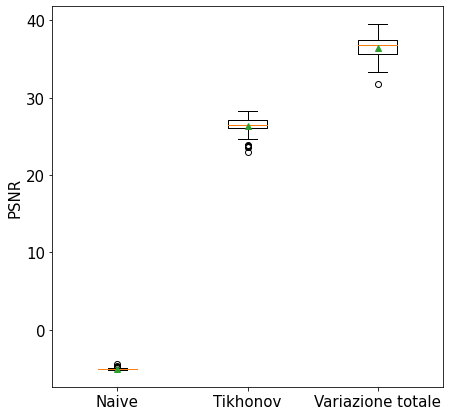
\includegraphics[width=6.5cm]{esecuzioni_multiple/100/psnr1.png}
        \label{fig:100_psnr1}
    \end{minipage}\hfill
    \begin{minipage}{0.45\textwidth}
        \centering
        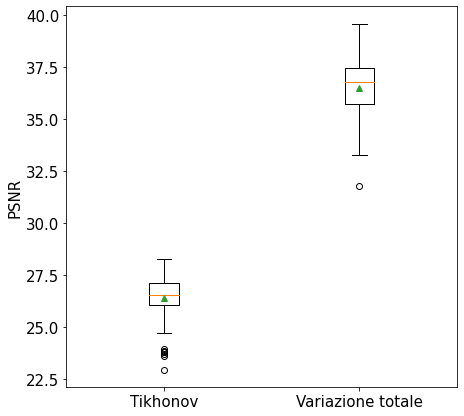
\includegraphics[width=6.5cm]{esecuzioni_multiple/100/psnr2.png}
        \label{fig:100_psnr2}
    \end{minipage}
    \caption{Boxplot per il PSNR}
\end{figure}
\begin{center}
    \begin{tabular}{ |c|c|c| }
    \hline
    & Tikhonov & Variazione totale \\ 
    \hline
    Intervallo (\emph{outlier} esclusi) & $[26.03, 28.25]$ & $[35.71, 39.58]$ \\
    Media & $26.39$ & $36.49$ \\
    Mediana & $26.53$ & $36.76$ \\
    Deviazione standard & $1.05$ & $1.38$ \\
    \hline
    \end{tabular}
\end{center}
In linea con i risultati precedenti, il metodo naive ha prodotto soluzioni non accettabili, 
mentre i metodi regolarizzati hanno avuto un comportamento migliore.\\
È evidente che i risultati ottenuti regolarizzando con variazione totale sono migliori rispetto a quelli ottenuti con Tikhonov. A livello di stabilità però, le soluzioni prodotte tramite variazione totali presentano, anche se di poco, valori di PSNR più sparsi rispetto a quelli di Tikhonov.

\begin{figure}[H]
    \centering
    \begin{minipage}{0.45\textwidth}
        \centering
        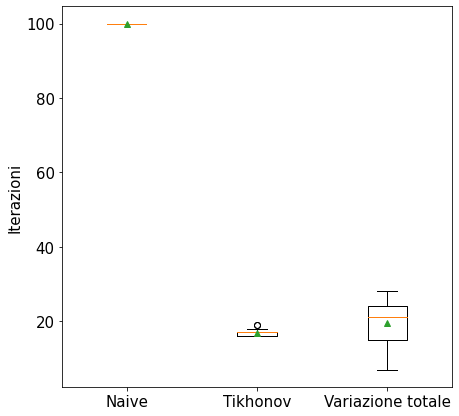
\includegraphics[width=6.5cm]{esecuzioni_multiple/100/iter1.png}
        \label{fig:100_iter1}
    \end{minipage}\hfill
    \begin{minipage}{0.45\textwidth}
        \centering
        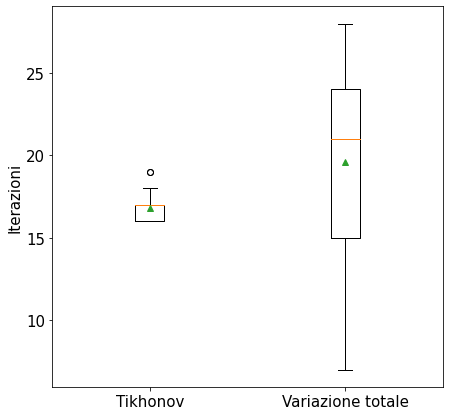
\includegraphics[width=6.5cm]{esecuzioni_multiple/100/iter2.png}
        \label{fig:100_iter2}
    \end{minipage}
    \caption{Boxplot per il numero di iterazioni}
\end{figure}

\begin{center}
    \begin{tabular}{ |c|c|c| }
    \hline
    & Tikhonov & Variazione totale \\ 
    \hline
    Intervallo (\emph{outlier} esclusi) & $[16, 18]$ & $[15, 28]$ \\
    Media & $16.79$ & $19.59$ \\
    Mediana & $17$ & $21$ \\
    Deviazione standard & $0.75$ & $5.47$ \\
    \hline
    \end{tabular}
\end{center}
Anche a livello di numero di iterazioni, il metodo naive ha avuto il risultato peggiore, terminando al raggiungimento del numero massimo di iterazioni.\\
La regolarizzazione di Tikhonov ha richiesto un numero di iterazioni contenuto e coerente, mentre la regolarizzazione tramite variazione totale ha mostrato dati più diradati e meno prevedibili come testimoniato dal valore della deviazione standard.\\
In linea di massima, considerando la complessità dei termini di regolarizzazione e gli esperimenti effettuati, il tempo di esecuzione richiesto per la regolarizzazione tramite variazione totale è in generale maggiore rispetto a Tikhonov.

\newpage
\subsection{Esecuzioni sul dataset}
Rispetto alle otto immagini contenute nel dataset utilizzato, sono state eseguite diverse misurazioni al variare della dimensione del kernel, del valore di $\sigma_{\text{kernel}}$ e della deviazione standard del rumore. 
Per tutte le esecuzioni è stato scelto il valore del parametro di regolarizzazione utilizzando lo stesso procedimento iterativo della \autoref{chap:lambda}.\\
I risultati in forma aggregata sono i seguenti:
\begin{center}
    \begin{tabular}{ |cc|c|c|c|c|c|c|c| }
    \hline
    \multicolumn{3}{|c|}{} & \multicolumn{3}{c|}{MSE} & \multicolumn{3}{c|}{PSNR} \\
    \hline
    \multicolumn{2}{|c|}{Kernel} & Noise & Naive & Tikhonov & Var. tot. & Naive & Tikhonov & Var. tot. \\ 
    \hline
	$7 \times 7$ & $\sigma=0.5$ & $\sigma=0.05$ & $0.19 \cdot 10^{0}$ & $0.40 \cdot 10^{-2}$ & $0.21 \cdot 10^{-3}$ & 7.14 & 24.16 & 36.94 \\
	$7 \times 7$ & $\sigma=1$ & $\sigma=0.05$ & $0.10 \cdot 10^{1}$ & $0.27 \cdot 10^{-2}$ & $0.24 \cdot 10^{-3}$ & -0.16 & 25.85 & 36.42 \\
    $7 \times 7$ & $\sigma=1.3$ & $\sigma=0.05$ & $0.76 \cdot 10^{0}$ & $0.24 \cdot 10^{-2}$ & $0.26 \cdot 10^{-3}$ & 1.21 & 26.36 & 36.07 \\
    $7 \times 7$ & $\sigma=3$ & $\sigma=0.05$ & $0.12 \cdot 10^{1}$ & $0.17 \cdot 10^{-2}$ & $0.34 \cdot 10^{-3}$ & -0.63 & 27.8 & 34.88 \\
	\hline
    $9 \times 9$ & $\sigma=0.5$ & $\sigma=0.05$ & $0.19 \cdot 10^{0}$ & $0.40 \cdot 10^{-2}$ & $0.21 \cdot 10^{-3}$ & 7.13 & 24.16 & 36.9 \\
	$9 \times 9$ & $\sigma=1$ & $\sigma=0.05$ & $0.10 \cdot 10^{1}$ & $0.27 \cdot 10^{-2}$ & $0.23 \cdot 10^{-3}$ & -0.17 & 25.85 & 36.42 \\
	$9 \times 9$ & $\sigma=1.3$ & $\sigma=0.05$ & $0.76 \cdot 10^{0}$ & $0.24 \cdot 10^{-2}$ & $0.25 \cdot 10^{-3}$ & 1.18 & 26.35 & 36.16 \\
    $9 \times 9$ & $\sigma=3$ & $\sigma=0.05$ & $0.53 \cdot 10^{0}$ & $0.17 \cdot 10^{-2}$ & $0.36 \cdot 10^{-3}$ & 2.73 & 27.77 & 34.68 \\
    \hline
    $25 \times 25$ & $\sigma=0.5$ & $\sigma=0.05$ & $0.42 \cdot 10^{0}$ & $0.37 \cdot 10^{-2}$ & $0.19 \cdot 10^{-3}$ & 3.81 & 24.48 & 37.21 \\
    $25 \times 25$ & $\sigma=1$ & $\sigma=0.05$ & $0.81 \cdot 10^{0}$ & $0.28 \cdot 10^{-2}$ & $0.23 \cdot 10^{-3}$ & 0.92 & 25.65 & 36.45 \\
    $25 \times 25$ & $\sigma=1.3$ & $\sigma=0.05$ & $0.78 \cdot 10^{0}$ & $0.25 \cdot 10^{-2}$ & $0.25 \cdot 10^{-3}$ & 1.09 & 26.21 & 36.16 \\
    $25 \times 25$ & $\sigma=3$ & $\sigma=0.05$ & $0.35 \cdot 10^{0}$ & $0.18 \cdot 10^{-2}$ & $0.35 \cdot 10^{-3}$ & 4.58 & 27.64 & 34.71 \\
    \hline
	$7 \times 7$ & $\sigma=3$ & $\sigma=0.2$ & $0.19 \cdot 10^{2}$ & $0.74 \cdot 10^{-2}$ & $0.88 \cdot 10^{-3}$ & -12.75 & 21.46 & 30.64 \\
	$9 \times 9$ & $\sigma=3$ & $\sigma=0.2$ & $0.88 \cdot 10^{1}$ & $0.71 \cdot 10^{-2}$ & $0.87 \cdot 10^{-3}$ & -9.46 & 21.63 & 30.7 \\
	$25 \times 25$ & $\sigma=3$ & $\sigma=0.2$ & $0.53 \cdot 10^{1}$ & $0.71 \cdot 10^{-2}$ & $0.90 \cdot 10^{-3}$ & -7.2 & 21.61 & 30.53 \\
	$51 \times 51$ & $\sigma=3$ & $\sigma=0.2$ & $0.52 \cdot 10^{1}$ & $0.71 \cdot 10^{-2}$ & $0.90 \cdot 10^{-3}$ & -7.19 & 21.63 & 30.51 \\
	$95 \times 95$ & $\sigma=3$ & $\sigma=0.2$ & $0.53 \cdot 10^{1}$ & $0.71 \cdot 10^{-2}$ & $0.90 \cdot 10^{-3}$ & -7.21 & 21.62 & 30.55 \\
    \hline
    \end{tabular}
\end{center}
Come in tutti i casi precedenti, la ricostruzione naive ha prodotto soluzioni completamente distanti dall'immagine reale.\\
Si nota che, variando la dimensione del kernel fissati $\sigma_{\text{kernel}}$ e $\sigma_{\text{noise}}$, il risultato ottenuto differisce tra i diversi casi di piccole quantità e non appaiono particolari correlazioni.\\
È evidente, invece, un fenomeno ricorrente nella precisione di ricostruzione per i metodi regolarizzati all'aumentare di $\sigma_{\text{kernel}}$: con Tikhonov la fedeltà della soluzione rispetto all'immagine reale è maggiore all'aumentare di $\sigma_{\text{kernel}}$, mentre per la variazione totale il fenomeno è inverso, generando una ricostruzione meno accurata.

\begin{center}
    \begin{tabular}{ |cc|c|c|c|c|c| }
    \hline
    & & & \multicolumn{2}{c|}{MSE} & \multicolumn{2}{c|}{PSNR} \\
    \hline
    \multicolumn{2}{|c|}{Kernel} & Noise & Tikhonov & Var. tot. & Tikhonov & Var. tot. \\ 
    \hline
    $9 \times 9$ & $\sigma=0.5$ & $\sigma=0.05$ & $0.40 \cdot 10^{-2}$ & $0.21 \cdot 10^{-3}$ & 24.16 & 36.9 \\
	$9 \times 9$ & $\sigma=1$ & $\sigma=0.05$ & $0.27 \cdot 10^{-2}$ & $0.23 \cdot 10^{-3}$ & 25.85 & 36.42 \\
	$9 \times 9$ & $\sigma=1.3$ & $\sigma=0.05$ & $0.24 \cdot 10^{-2}$ & $0.25 \cdot 10^{-3}$ & 26.35 & 36.16 \\
    $9 \times 9$ & $\sigma=3$ & $\sigma=0.05$ & $0.17 \cdot 10^{-2}$ & $0.36 \cdot 10^{-3}$ & 27.77 & 34.68 \\
    $9 \times 9$ & $\sigma=4$ & $\sigma=0.05$ & $0.16 \cdot 10^{-2}$ & $0.39 \cdot 10^{-3}$ & 28.14 & 34.24 \\
    $9 \times 9$ & $\sigma=5$ & $\sigma=0.05$ & $0.15 \cdot 10^{-2}$ & $0.42 \cdot 10^{-3}$ & 28.31 & 33.85 \\
    $9 \times 9$ & $\sigma=10$ & $\sigma=0.05$ & $0.17 \cdot 10^{-2}$ & $0.58 \cdot 10^{-3}$ & 27.97 & 32.55 \\
    $9 \times 9$ & $\sigma=15$ & $\sigma=0.05$ & $0.18 \cdot 10^{-2}$ & $0.58 \cdot 10^{-3}$ & 27.71 & 32.52 \\
    $9 \times 9$ & $\sigma=30$ & $\sigma=0.05$ & $0.19 \cdot 10^{-2}$ & $0.59 \cdot 10^{-3}$ & 27.36 & 32.43 \\
    $9 \times 9$ & $\sigma=60$ & $\sigma=0.05$ & $0.20 \cdot 10^{-2}$ & $0.64 \cdot 10^{-3}$ & 27.19 & 32.1 \\
    $9 \times 9$ & $\sigma=100$ & $\sigma=0.05$ & $0.21 \cdot 10^{-2}$ & $0.59 \cdot 10^{-3}$ & 27.08 & 32.42 \\
	$9 \times 9$ & $\sigma=200$ & $\sigma=0.05$ & $0.21 \cdot 10^{-2}$ & $0.61 \cdot 10^{-3}$ & 27.04 & 32.29 \\
	\hline
    \end{tabular}
\end{center}

Analizzando più nel dettaglio il fenomeno, fissata una dimensione del kernel e variando il valore di $\sigma_{\text{kernel}}$, si nota lo stesso comportamento visto in \autoref{chap:lambda}.\\
Il risultato prodotto da Tikhonov, su immagini a cui è stato applicato un blur di ordini di grandezza contenuti, produce una soluzione molto simile all'immagine acquisita, 
mentre aumentando il fattore di blur, il risultato tende ad essere migliore fino ad una soglia dopo la quale inizia a descrescere.\\
Il metodo tramite variazione totale, invece, ha un comportamento più lineare e all'aumentare di $\sigma_{\text{kernel}}$ decresce la qualità della ricostruzione.




\newpage
\section{Risultati su immagini complesse}

\subsection{Notte Stellata}
Utilizzando un blur con kernel $9 \times 9$, $\sigma=0.5$ e un rumore con deviazione standard $0.05$:
\begin{figure}[H]
    \centering
    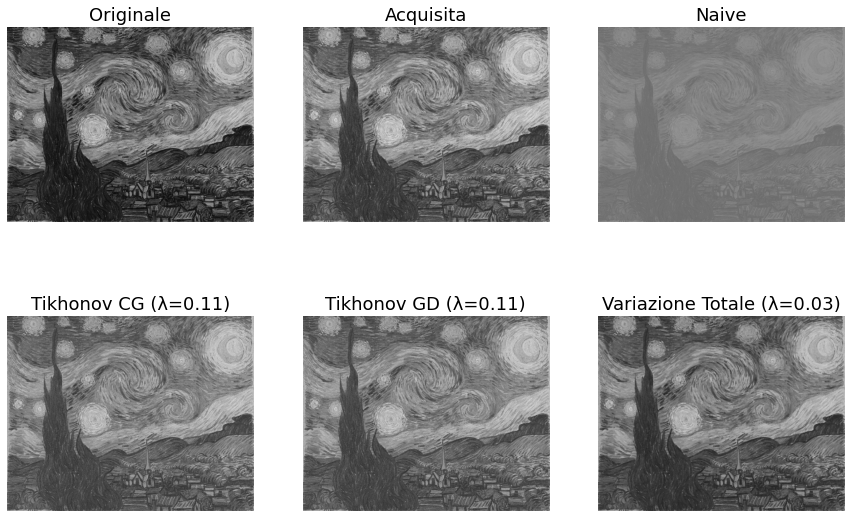
\includegraphics[width=11cm]{reale/1/1/deblur.png}
    \caption{Deblur applicato sulla Notte Stellata}
    \label{fig:deblur_reale1_1}
\end{figure}
\begin{center}
    \begin{tabular}{ |c|c|c|c|c|c| }
    \hline
    & Acquisita & Naive & Tikhonov & Variazione totale \\ 
    \hline
    MSE & $0.531 \cdot 10^{-2}$ & $0.204 \cdot 10^{0}$ & $0.712 \cdot 10^{-2}$ & $0.502 \cdot 10^{-2}$ \\ 
    PSNR & $22.75$ & $6.91$ & $21.47$ & $22.99$ \\ 
    \hline
    \end{tabular}
\end{center}

Utilizzando un blur con kernel $25 \times 25$, $\sigma=3$ e un rumore con deviazione standard $0.1$:
\begin{figure}[H]
    \centering
    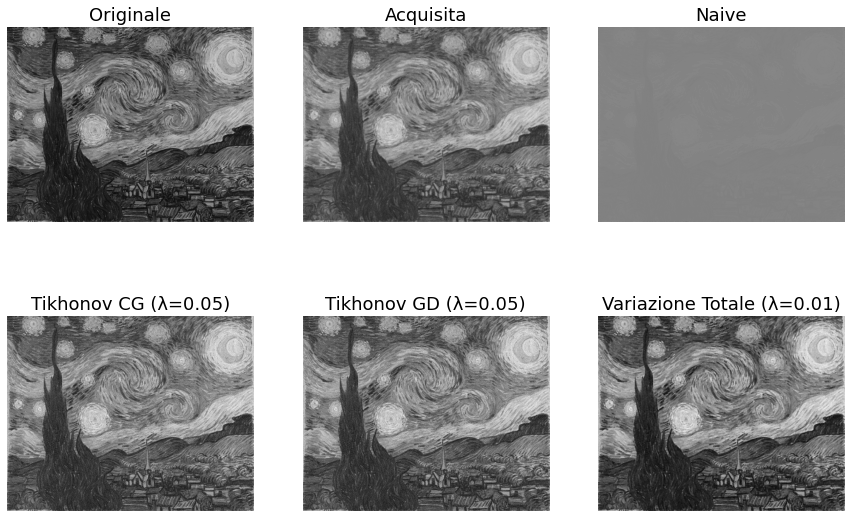
\includegraphics[width=11cm]{reale/1/2/deblur.png}
    \caption{Deblur applicato sulla Notte Stellata}
    \label{fig:deblur_reale1_2}
\end{figure}
\begin{center}
    \begin{tabular}{ |c|c|c|c|c|c| }
    \hline
    & Acquisita & Naive & Tikhonov & Variazione totale \\ 
    \hline
    MSE & $0.173 \cdot 10^{-1}$ & $0.212 \cdot 10^{2}$ & $0.105 \cdot 10^{-1}$ & $0.818 \cdot 10^{-2}$ \\ 
    PSNR & $17.61$ & $-13.26$ & $19.80$ & $20.87$ \\ 
    \hline
    \end{tabular}
\end{center}

\subsubsection{Analisi}
Come già osservato più volte, il risultato ottenuto con il metodo naive in tutti i casi è molto instabile, 
mentre con Tikhonov vengono prodotti risultati significativi con valori di $\sigma_{\text{kernel}}$ non troppo piccoli.\\
Per la regolarizzazione tramite variazione totale, invece, a differenza dei casi precedentemente analizzati, ha sempre prodotto la soluzione migliore ma con valori di PSNR molto vicini all'immagine corrotta nel primo caso e non troppo distanti da Tikhonov nel secondo.
È inoltre possibile osservare il problema di semi-convergenza in una forma molto contenuta:
\begin{figure}[H]
    \centering
    \begin{minipage}{0.45\textwidth}
        \centering
        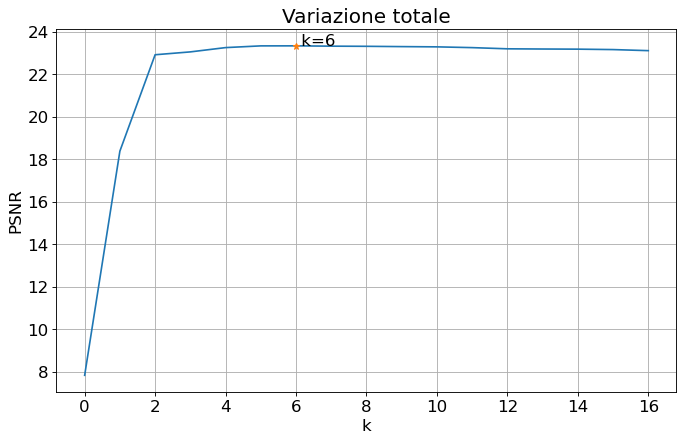
\includegraphics[width=7cm]{reale/1/1/tv_semiconvergenza.png}
        \caption{PSNR per la $1^{\text{a}}$ esecuzione}
    \label{fig:semiconvergenza_reale1_1}
    \end{minipage}\hfill
    \begin{minipage}{0.45\textwidth}
        \centering
        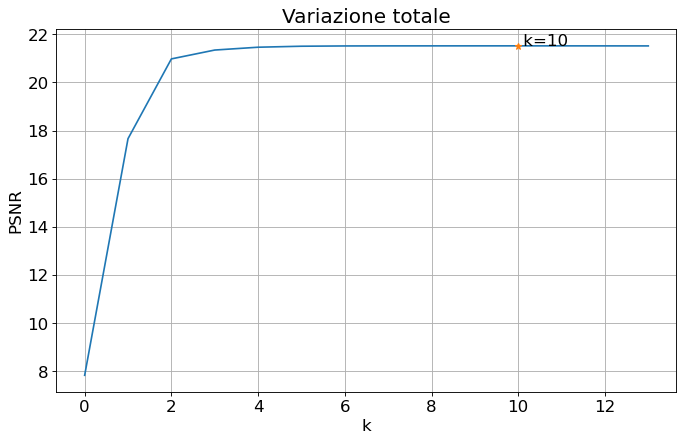
\includegraphics[width=7cm]{reale/1/2/tv_semiconvergenza.png}
        \caption{PSNR per la $2^{\text{a}}$ esecuzione}
    \label{fig:semiconvergenza_reale1_2}
    \end{minipage}
\end{figure}

\subsection{Cielo stellato}
Utilizzando un blur con kernel $25 \times 25$, $\sigma=3$ e un rumore con deviazione standard $0.05$:
\begin{figure}[H]
    \centering
    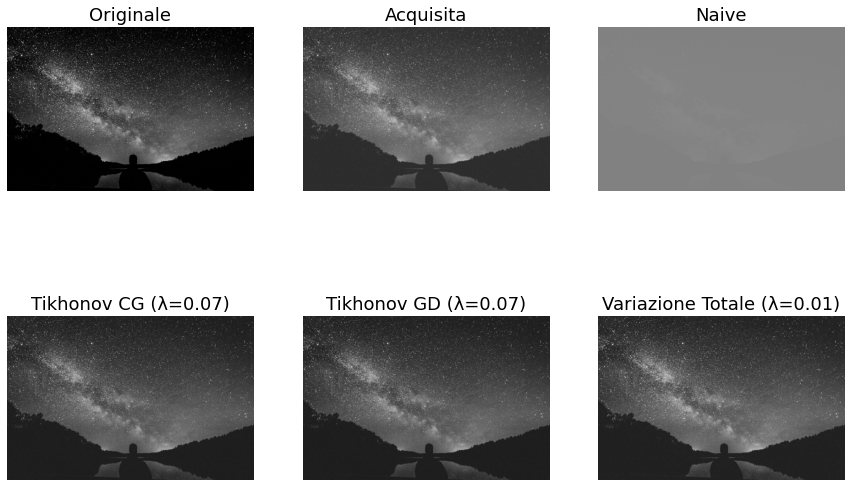
\includegraphics[width=15cm]{reale/2/deblur.png}
    \caption{Deblur applicato sul cielo stellato}
    \label{fig:deblur_reale2}
\end{figure}
\begin{center}
    \begin{tabular}{ |c|c|c|c|c|c| }
    \hline
    & Acquisita & Naive & Tikhonov & Variazione totale \\ 
    \hline
    MSE & $0.567 \cdot 10^{-2}$ & $0.524 \cdot 10^{1}$ & $0.35 \cdot 10^{-2}$ & $0.289 \cdot 10^{-2}$ \\ 
    PSNR & $22.47$ & $-7.19$ & $24.55$ & $25.39$ \\ 
    \hline
    \end{tabular}
\end{center}

\subsubsection{Analisi}
Anche in questo caso, il risultato ottenuto è del tutto simile alle analisi precedenti.\\
Non utilizzando più immagini "semplici", i metodi regolarizzati hanno prodotto risultati molto simili, anche se comunque la variazione totale presenta soluzioni migliori.\\
Un aspetto particolare di questa esecuzione è che la semiconvergenza della regolarizzazione di Tikhonov ha assunto un comportamento simile a quello della variazione totale:
\begin{figure}[H]
    \centering
    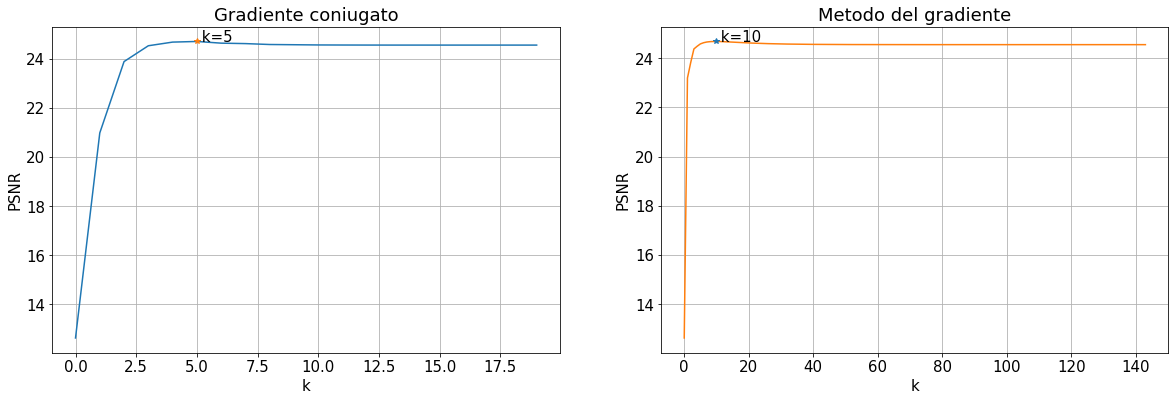
\includegraphics[width=15cm]{reale/2/tikhonov_semiconvergenza.png}
    \caption{Variazione del PSNR per Tikhonov}
    \label{fig:semiconvergenza_tikhonov_reale2}
\end{figure}
\begin{figure}[H]
    \centering
    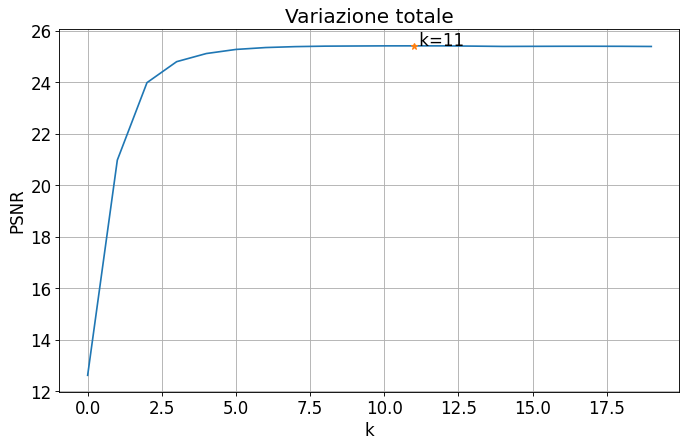
\includegraphics[width=8cm]{reale/2/tv_semiconvergenza.png}
    \caption{Variazione del PSNR per la variazione totale}
    \label{fig:semiconvergenza_tv_reale2}
\end{figure}


\newpage
\section{Conclusioni}
\subsection{Metodo naive}
Si può confermare che il processo di deblur risolvendo il problema ai minimi quadrati senza regolarizzazione è una soluzione estremamente mal condizionata e inaffidabile che richiede anche un numero di iterazioni molto elevato per raggiungere convergenza.\\
Utilizzando un'immagine che non è soggetta a rumore, invece, il risultato prodotto è molto vicino a quello reale e tende ad essere un approccio migliore rispetto ai metodi regolarizzati.

\subsection{Regolarizzazione di Tikhonov}
Il metodo di regolarizzazione di Tikhonov si è rivelato utile su immagini con un blur di determinati ordini di grandezza. 
Infatti, se il blur è molto contenuto, la soluzione prodotta tende ad essere del tutto simile all'immagine acquisita, mentre per valori di blur più elevati si riesce a produrre un risultato più vicino all'immagine reale.\\
In termini di prestazioni invece, il metodo converge in un numero di iterazioni non troppo variabile e in tempo contenuto.

\subsection{Regolarizzazione tramite variazione totale}
Il metodo di regolarizzazione tramite variazione totale è invece il metodo che, tra quelli utilizzati, produce la soluzione migliore.\\
A differenza degli altri metodi, si è notato che è soggetto al problema di semi-convergenza in modo molto controllato e produce in tutti i casi analizzati una buona approssimazione dell'immagine reale.\\
A livello di velocità, il numero di iterazioni richiesto in forma aggregata ha prodotto una deviazione standard abbastanza elevata e per questo tende a non essere prevedibile. 
Anche sperimentalmente, il tempo di esecuzione è solitamente stato maggiore rispetto a Tikhonov.\\
Bisogna anche ricordare che applicato a immagini più complesse, il metodo ha prodotto ricostruzioni qualitativamente meno vicine alla realtà ed è stato analizzato un caso in cui la soluzione era molto simile a quella prodotta da Tikhonov. Ciò apre a scenari in cui, nonostante la variazione totale produca soluzioni migliori, è potenzialmente più conveniente optare per la regolarizzazione di Tikhonov.




\newpage
\printbibliography[title={Bibliografia}]

\end{document}
